%\toggletrue{ownans}
\qitem{%
    \noindent\begin{minipage}{.6\linewidth}
        Treating each of the balls in the figure below as distinct, how many ways are there to select 3 balls from the same horizontal row?
    \end{minipage}
    \begin{minipage}{.4\linewidth}
        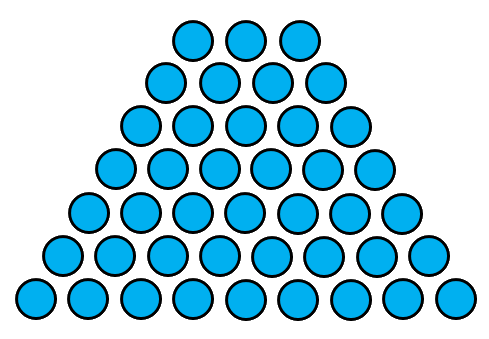
\includegraphics[width=\linewidth]{../dgs2020/co3_pic/Amot-grouping-balls.png}
    \end{minipage}
    }{%
    The smallest row has 3 balls and the largest row has 9 balls. The number of ways to select 3 balls from the same row can be expressed as a sum of binomial coefficients. This can then be computed with the hockey stick identity:
    \[\sum\limits_{k=3}^{9}\binom{k}{3} = \binom{10}{4} = 210.\]
    So, there are 210 ways to select 3 balls from the same row.
    }{%
    https://brilliant.org/wiki/hockey-stick-identity/
}

\qitem{%
    In Pascal's Triangle, each entry is the sum of the two entries above it. In which row of Pascal's Triangle do three consecutive entries occur that are in the ratio $3: 4: 5$?
    }{%
    Consider what the ratio means. Since we know that they are consecutive terms, we can say \[\frac{\dbinom{n}{k-1}}{3} = \frac{\dbinom{n}{k}}{4} = \frac{\dbinom{n}{k+1}}{5}.\]

    Taking the first part, and using our expression for $n$ choose $k$, \[\frac{n!}{3(k-1)!(n-k+1)!} = \frac{n!}{4k!(n-k)!}\] \[\frac{1}{3(n-k+1)} = \frac{1}{4k}\] \[n-k+1 = \frac{4k}{3}\] \[\frac{3(n+1)}{7} = k\] 
    Then, we can use the second part of the equation. 
    \[\frac{n!}{4k!(n-k)!} = \frac{n!}{5(k+1)!(n-k-1)!}\] 
    \[\frac{1}{4(n-k)} = \frac{1}{5(k+1)}\] 
    \[\frac{4(n-k)}{5} = k+1\] 
    \[\frac{4n}{5} = \frac{9k}{5} +1.\] 
    Since we know $k = \frac{3(n+1)}{7}$ we can plug this in, giving us \[\frac{4n}{5} = \frac{9\left(\frac{3(n+1)}{7}\right)}{5} +1\] \[7(4n - 5) = 27n+27\] \[n = 62.\] We can also evaluate for $k$, and find that $k = \frac{3(62+1)}{7} = 27.$ Since we want $n$, however, our final answer is $\boxed{062.}$
    }{%
    https://artofproblemsolving.com/wiki/index.php/Pascal_Triangle_Related_Problems
    https://artofproblemsolving.com/wiki/index.php/1992_AIME_Problems/Problem_4
}

\qitem{%
    Melinda has three empty boxes and $12$ textbooks, three of which are mathematics textbooks. One box will hold any three of her textbooks, one will hold any four of her textbooks, and one will hold any five of her textbooks. If Melinda packs her textbooks into these boxes in random order, the probability that all three mathematics textbooks end up in the same box can be written as $\frac{m}{n}$, where $m$ and $n$ are relatively prime positive integers. Find $m+n$.
    }{%
    Consider the books as either math or not-math where books in each category are indistiguishable from one another. Then, there are $\,_{12}C_{3}$ total distinguishable ways to pack the books. Now, in order to determine the desired propability, we must find the total number of ways the condition that all math books are in the same box can be satisfied. We proceed with casework for each box:

    Case 1: The math books are placed into the smallest box. This can be done in $\binom{3}{3}$ ways.

    Case 2: The math books are placed into the middle box. This can be done in $\binom{4}{3}$ ways.

    Case 3: The math books are placed into the largest box. This can be done in $\binom{5}{3}$ ways.

    So, the total ways the condition can be satisfied is $\binom{3}{3} + \binom{4}{3} + \binom{5}{3}$. This can be simplified to $\binom{6}{4} = \binom{6}{2}$ by the Hockey Stick Identity. Therefore, the desired probability is $\dfrac{\dbinom{6}{2} }{\dbinom{12}{3}}$ = $\dfrac{3}{44}$, and $m+n=3+44=\boxed{047}$.
    }{%
    https://artofproblemsolving.com/wiki/index.php?title=2013_AIME_I_Problems/Problem_6#Solution_Two
}

